% A good introduction to latex can be found here:
%  http://www.cse.ohio-state.edu/~hank/latex/lshort141.pdf

\documentclass{article}
\usepackage{amsmath}

\usepackage{full page}  % make the margins somewhat smaller than the default

\usepackage{listings}  %  needed for source code listings
\usepackage{color}
\usepackage{hyperref}
\usepackage{graphicx}
\usepackage[tight,footnotesize]{subfigure}

\definecolor{javared}{rgb}{0.7,0,0} % for strings
\definecolor{javagreen}{rgb}{0.25,0.6,0.35} % comments
\definecolor{javapurple}{rgb}{0.55,0,0.40} % keywords
\definecolor{javadocblue}{rgb}{0.25,0.35,0.85} % javadoc

\definecolor{pblue}{rgb}{0.13,0.13,1}
\definecolor{pgreen}{rgb}{0,0.5,0}
\definecolor{pred}{rgb}{0.9,0,0}
\definecolor{pgrey}{rgb}{0.46,0.45,0.48}
 
\lstset{language=Java,
basicstyle=\ttfamily,
  commentstyle=\color{pgreen},
  keywordstyle=\color{pblue},
  stringstyle=\color{pred},
morecomment=[s][\color{javadocblue}]{/**}{*/},
numbers=left,
numberstyle=\tiny\color{black},
stepnumber=2,
numbersep=10pt,
tabsize=4,
showspaces=false,
showstringspaces=false,
frame=shadowbox,
numbers=left,
%escapechar=\@
} 

% set the document title, author, and date here.
%  once set, the \maketitle command (within the document)
%  will display them nicely
\title{Chess AI}
\author{Junjie Guan $<gjj@cs.dartmouth.edu>$}

\begin{document}
\maketitle

\tableofcontents

\section{Introduction}

\emph{`Constraint satisfaction problems (CSPs) are mathematical problems defined as a set of objects whose state must satisfy a number of constraints or limitations.'}\footnote{Wikipedia: \url{http://en.wikipedia.org/wiki/Constraint_satisfaction_problem}}













\clearpage
\section{Overview}
\subsection{Problem defination}
CSP is usually defined  with a tuple $<X, D, C>$, as following:
$$X = \{X_1, ..., X_n\}$$
$$D = \{D_1, ..., D_k\}$$
$$C = \{C_1, ..., C_m\}$$
where  $X$, $D$ and $C$ is a set of variables, domains and constraints. Our goal is to assign each variable a non-empty domain value from $D$, while satisfying all the constraints in $C$.

\subsection{Design Layout}
Figure \ref{classlayout} is an overview my codes design. Basically it can be devided into 3 parts.  

\begin{itemize}
  \item The drivers contains the main function that read the input dataset and present the results/solutions.
  \item  The second part is problem defination, theasf the asdf. It contains the basic definition of CSP problem. For example, the Variable, Constraints represent the the set I mentioned above, with necessary methods inside. Such as building constraints, validating the assignment, etc. I implement most of the method in a generic class, while I also extend the basic class for the needs of different problem. Despite of this, solver do not care about the specific problem. It only deal with those lower generic classes.
  \item The third part the problem solver, where I implement the CSP algorihtm that solves the problem, as well as some helper methods such as heuristic compuation.
\end{itemize}
\begin{figure*}[!h]
\centering
\includegraphics[width=0.99\textwidth]{class_layout.png}
\caption{Overview of the design}
\label{classlayout}
\end{figure*}







\subsubsection{minimaxIDS}

\textbf{minimaxIDS} initializes the search using iterative-depending strategy.


\begin{lstlisting}[numbers=left]
private short minimaxIDS(Position position, int maxDepth) 
    throws IllegalMoveException{
  this.terminalFound = false;
  MoveValuePair bestMove = new MoveValuePair();
  for (int d = 1; d <= maxDepth && !this.terminalFound; d++) {
    bestMove = maxMinValue(position, maxDepth - 1, MAX_TURN);
  }
  return bestMove.move;
}
\end{lstlisting}


\subsubsection{maxMinValue}

\textbf{maxMinValue} is an recursive funciton that keep searching in the tree. I write it in a compact way by mering min and max procedure in this one method, which turns out to be a big mistake for future when I try to implement more fancy mechansim for the searching. This design makes the codes a little messy.

There is also another better way to implement the search in a compact way, which is called \emph{Nagamax}. However it was too late for me to discover it so I leave it to my future work.

\begin{lstlisting}[numbers=left]
private MoveValuePair maxMinValue(Position position, int depth, 
    boolean maxTurn) throws IllegalMoveException{
  if (depth <= 0 || position.isTerminal()) {
    // the base case of recursion
    return handleTerminal(position, maxTurn);
  } else {
    // get all the legal moves
    MoveValuePair bestMove = new MoveValuePair();
    for (short move : position.getAllMoves()) {
      // collect values from further moves by recursion
      position.doMove(move);
      MoveValuePair childMove = maxMinValue(position, depth - 1, !maxTurn);
      bestMove.updateMinMax(move, childMove.eval, maxTurn);
      position.undoMove();
    }
    return bestMove;
  }
}
\end{lstlisting}

\subsubsection{handleTerminal}

\textbf{handleTerminal} is used to terminate the searching by returning an evalution value, when either reaching the maximun depth or check mate or draw. Noted that getMaterial evalutes the weighted sum of the stones, while getDominant evaluates the distribution of the stones.

\begin{lstlisting}[numbers=left]
private MoveValuePair handleTerminal(Position position, boolean maxTurn) {
  MoveValuePair finalMove = new MoveValuePair();
  if (position.isTerminal() && position.isMate()) {
    this.terminalFound = position.isTerminal();
    finalMove.eval = (maxTurn ? BE_MATED : MATE);
  } else if (position.isTerminal() && position.isStaleMate())
     finalMove.eval = 0;
  else {
    finalMove.eval = (int) ( (maxTurn ? 1 : -1) * (position.getMaterial() 
       + position.getDomination()));
  }
  return finalMove;
}
\end{lstlisting}

\subsubsection{helper class}

\textbf{MoveValuePair} help me to store the move and corresponding evaluation value. Also it has a generalized method that help me to find the max value for maximum search, or vise versa.

\begin{lstlisting}[numbers=left]
private MoveValuePair handleTerminal(Position position, boolean maxTurn) {
  MoveValuePair finalMove = new MoveValuePair();
  if (position.isTerminal() && position.isMate()) {
    this.terminalFound = position.isTerminal();
    finalMove.eval = (maxTurn ? BE_MATED : MATE);
  } else if (position.isTerminal() && position.isStaleMate())
     finalMove.eval = 0;
  else {
    finalMove.eval = (maxTurn ? 1 : -1) * position.getMaterial();
  }
  return finalMove;
}
\end{lstlisting}





























\clearpage
\section{Results demonstration}


I did a lot of testing, turn out that I don't leave myself much time to organize how to present them. Here I am going to focus on computation time of each step. I create a fix random seed for the random AI, and let my AI play with it. 

Figure \ref{miniab} demonstrate the step and time curve, with my Minimax against Random AI (blue curve),  $\alpha\beta$ pruning against Random AI respectively (green curve). The left figure is a normal plot, while y axis of the right one is set to log scale (Noted that logy scale will shrink the difference on $y$ direction!). Considering sometimes the computation time grows exponentially with depth, this can provide a better observation. As you can see, the $\alpha\beta$ pruning finish the game using exact same amount of steps, while taking much less computation time.

\begin{figure*}[!h]
% ensure that we have normalsize text
\normalsize
% Store the current equation number.
% Set the equation number to one less than the one
% desired for the first equation here.
% The value here will have to changed if equations
% are added or removed prior to the place these
% equations are referenced in the main text.
\centering
\subfigure[normal]{
\label{m-1-3} %% label for first subfigure
\includegraphics[width=0.48\textwidth]{mini_ab.eps}}
\subfigure[log scale]{
\label{m-1-0} %% label for second subfigure
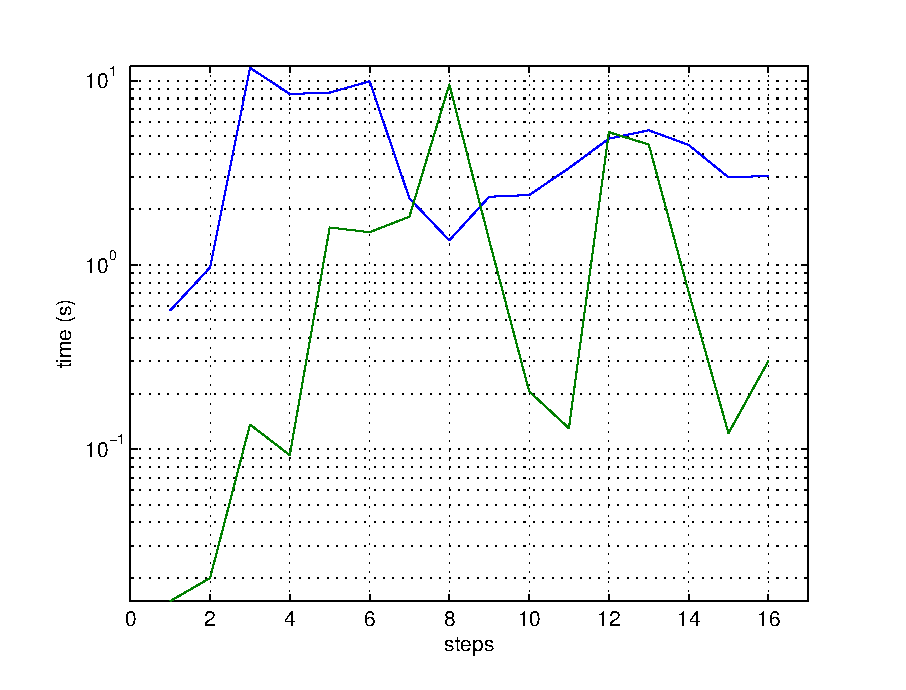
\includegraphics[width=0.48\textwidth]{mini_ab2.eps}}
\caption{step and time curve of Random MinimaxAI and $\alpha\beta$ pruning.}
\label{miniab} %% label for entire figure
\end{figure*}

Figure \ref{abtrans} demonstrate the step and time curve difference when there exists a tranposition table. As expected, the time conusmption is lower when implemented with transposition table. What's more, with transposition table it actually finish the game even fater! Because sometimes the table provider more depth of information than current node, which might lead to a bette decision.

Figure \ref{transorder} demonstrate the step and time curve difference when there exists a tranposition table. Though the time decrease even more significantly, the takes more steps for some unknown reason. I also test ordering enhancement against pure transposition table, it shows that after reodering it becomes a little more stupid. This leave as my future work.

Figure \ref{meantime} demonstrate mean time of different methods. It seems that null-move actually takes more time. I think it becuase although it reduce depth of search occassionally, it actually increase searching times on the same depth. May be I haven't tuned it properly. 

\begin{figure*}[!h]
\centering
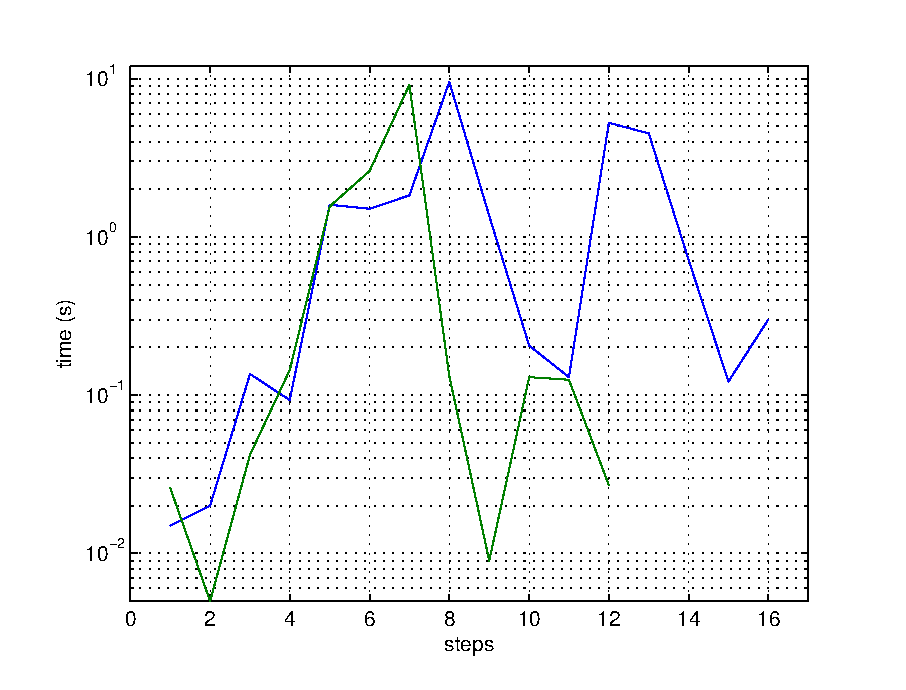
\includegraphics[width=0.48\textwidth]{mini_trans.eps}
\caption{step and time curve of $\alpha\beta$ pruning and$\alpha\beta$ enhanced with transposition table }
\label{abtrans}
\end{figure*}

\begin{figure*}[!h]
\centering
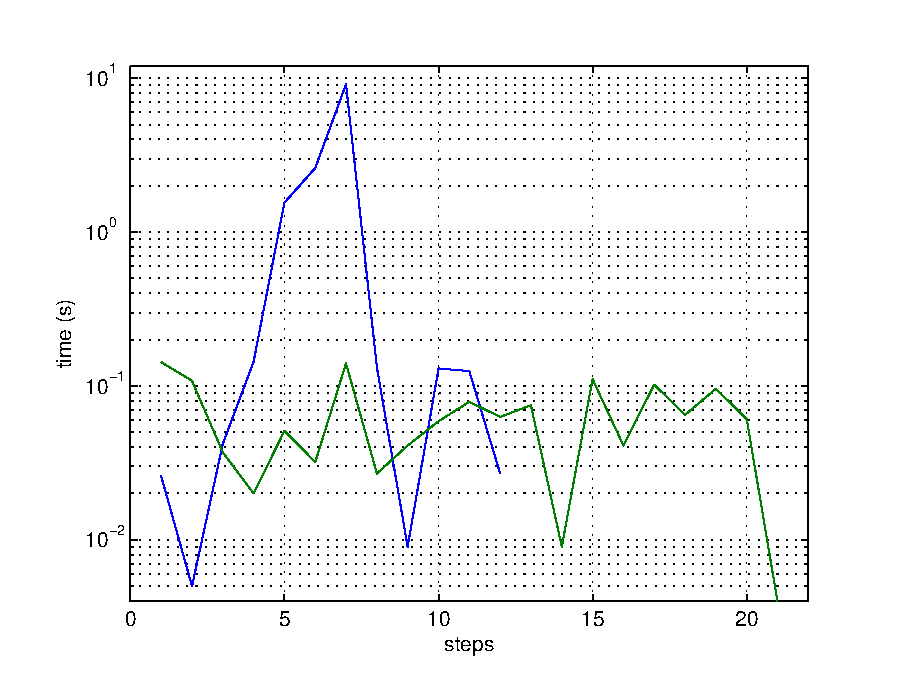
\includegraphics[width=0.48\textwidth]{trans_order.eps}
\caption{step and time curve of transposition table and$\alpha\beta$ enhanced with re-ordering}
\label{transorder}
\end{figure*}

\begin{figure*}[!h]
\centering
\includegraphics[width=0.48\textwidth]{meantime.eps}
\caption{mean time regards to Minimax, Alpha-beta pruning, transposition table, moves reodering, quiescence search and null move heuristic  repectively}
\label{meantime}
\end{figure*}


\clearpage
\section{Some related work}

Null move strategy can be very tricky. Adaptive Null-Move Pruning \footnote{Heinz, Ernst A. "Adaptive null-move pruning." Scalable Search in Computer Chess. Vieweg+ Teubner Verlag, 2000. 29-40.} prose some good suggestions. 1) when depth is less or equal to 6, use $R=2$. When Depth is larger than 8, use $R=3$. When depth is 6 or 7, and both sides has more than 3 stones, then $R = 3$. Otherwise, R = 2.




\end{document}